\chapter{Modules systèmes}
\label{ch:module_systems}


% Une bibliothèque de code est le regroupement de plusieurs types de données, des
% entiers, des nombres à virgule flottant, des chaînes de caractères, des
% fonctions et des données composites. L'ensemble de ces données constitue les
% fonctionnalités de la bibliothèque.

% Les fonctionnalités d'une bibliothèque
% peut être copié dans l'exécutable (bibliothèque statique), cela facilité la
% déploiement puisque que ses dépendances sont inclus dans un seul
% fichier.

Les bibliothèques au sein de systèmes de modules ont plusieurs formes.  Ils
peuvent être dans le langage source ou compilé dans un format natif. Le format
de bibliothèque étudié dans ce chapitre est le format natif du système
d'exploitation. Plus précisément, les bibliothèques dynamiques et leurs
interactions au sein d'un programme. Les formats des fichiers utilisés pour
les bibliothèques varient entre les différents systèmes d'exploitation.
Le système d'exploitation Linux utilise le format ELF (\textit{Extensible Linking
Format}), Microsoft Window utilise le format PE (\textit{Portable Executable})
et MacOSX utilise le format Mach-O (\textit{Mach object}) pour les exécutables
et les bibliothèques. L'utilisation d'une bibliothèque dynamique ce fait par
l'édition de liens durant l'exécution d'un programme.
% XXX: bytecodes aussi pour les langage compilé.

%Les langages
%de programmation interprétés fournisse leurs bibliothèques directement
%en code source. Dans cette catégorie, il y a Ruby, Python, Perl, Lua et
%Scheme -- dont le code des bibliothèques est écrit et frounit dans le
%langage respectif. Les langages compilés -- comme C, C++, C\# et Java --
%utilisent plutôt des formats binaires destiné, soit à une machine virtuelle
%(e.g. la \textit{Java Virtual Machine} JVM ou un architecture
%physique (e.g. i686, x86\_64, ARM). Les bibliothèques natives peuvent
%être utilisé


\section{Édition de liens dynamique}

Une application qui utilise une bibliothèque partagés ne contient pas le code
de la bibliothèque, mais plutôt le nom des fonctionnalités utilisés.  La
routine qui récupère la fonctionnalité à partir du nom est la
résolution qui est effectué par le \textit{dynamic loader}.  Lorsqu'un
programme lié dynamiquement à plusieurs bibliothèques partagés exécute invoque
une procédure externe, la routine de résolution est démarrée pour résoudre le
code de cette procédure.

%% Bibiothèque dynamique native.
Par exemple, sous Linux l'utilitaire <<yes>>, qui est écrit en C,
est lié aux bibliothèques systèmes suivantes:
\begin{verbatim}
  linux-vdso.so.1 (0x00007ffeef7f9000)
  libc.so.6 => /usr/lib/libc.so.6 (0x00007ff68161c000)
  /lib64/ld-linux-x86-64.so.2 => ...
\end{verbatim}

La bibliothèque \textit{libc.so.6} contient la plupart des fonctions standards
du système sous Linux.  Le chargement des bibliothèques s'effectue au début de
l'application, avant l'exécution de la fonction principale souvent nommé
\textbf{main}. Plusieurs bibliothèques peuvent coexister simultanément au sein
d'un même processus sans que l'exécution du programme en soit affecté.

La résolution des fonctionnalités de ces bibliothèques est effectuée par un
programme adapté le \textit{program interpreter} du système qui correspond à
\textit{/lib64/ld-linux-x86-64.so.2}.  Il est possible de forcer la résolution
d'une fonctionnalité d'une bibliothèque de façon manuel. Ce genre d'interaction
est possible sur les trois principales plateformes utilisées sur le marché
(Windows, MacOSX et Linux).

%% TODO: continue here FIXME
Sur Linux, l'API qui permet d'interagir avec les bibliothèques partagés provient de \textit{libdl.so}.
Elle contient les fonctions \textit{dlopen}, \textit{dlsym}, \textit{dlerror} et \textit{dlclose} pour gérer
des bibliothèques de code supplémentaire chargé manuellement à l'exécution.  Pour charger la fonction
\textit{foo}, qui ne prend pas d'argument et ne retourne rien de la bibliothèque \textit{libFoo.so} en C,
il faut exécuter les deux appels suivant:
\begin{center}
  \begin{figure}[ht]
\begin{lstlisting}[language=C,frame=single]
  ...
  void *handle = dlopen("./libFoo.so", RTLD_LAZY);
  void (*foo)() = dlsym(handle, "foo");
  ...
\end{lstlisting}
\caption{Chargement dynamique de la bibliothèque \textit{libFoo.so} et
résolution de la fonction \textit{foo} sans gestion d'erreur sous Linux}
  \end{figure}
\end{center}
L'équivalent des bibliothèques partagés sous Window sont les DLLs, ils peuvent être chargé de façon similaire dans un
programme en utilisant les fonctions \textit{LoadLibrary}, \textit{LoadLibraryEx} et \textit{GetProcAddress}. Ils
fonctionne de la même façon que leur équivalent Linux. Pour MacOSX, il faut passer par les routines:
\begin{itemize}
    \item \textit{NSCreateObjectFileImageFromFile}
    \item \textit{NSLinkModule}
    \item \textit{NSLookupSymbolInModule}
    \item \textit{NSAddressOfSymbol}
\end{itemize}

La majorité des langages interprétés permettent l'importation de bibliothèque
de code native, via un interface nommé \textit{foreign function interface}.
Cette interface offre une couche d'abstraction de ces procédures.
Prenons comme exemple les langage Python, Ruby, Lua et Scheme. Python possède
le module \textbf{ctypes} qui permet de chargé des bibliothèques natives dynamique, Ruby
possède le module \textbf{ffi}.
%Ces modules ne font qu'encapsuler les fonction de chargement de bibliotheques
%native pour qu'il puisse être invoqué dans le langage cible.

% Bibliothèque Lua en C
% - La bibliothèque doit avoir le même nom que celui utilisé par le \textit{import}.

Certains langages ont un mécanisme pour charger des bibliothèques natives s'ils
ont été conçus spécialement.  Dans le langage de programmation Lua, il est
possible chargé directement une bibliothèque dynamique si elle contient une
fonction \textbf{luaopen\_\textit{libname}} où \textit{libname} est le nom de
la bibliothèque.  Gambit Scheme utilise un mécanisme équivalent. Il permet le
chargement de ces modules qui ont été compilé en bibliothèque partagé (DLL)
avec la fonction \textit{(\textbf{load} "libname")}.

%% Python
%\begin{figure}[ht]
%\begin{lstlisting}[language=python,frame=single]
%# From https://docs.python.org/2/library/ctypes.html
%from ctypes import *
%# Chargement d'une bibliotheque native.
%lib = cdll.LoadLibrary("./libFoo.so")
%# Appel de la fonction foo.
%lib.foo()
%\end{lstlisting}
%\caption{Code d'importation de la fonction \textbf{foo} de la bibliothèque \textit{libFoo.so} en Python}
%\end{figure}

\begin{center}
% Ruby
\begin{figure}[ht]
\begin{lstlisting}[language=ruby,frame=single]
require 'ffi'
# Chargement d'une bibliotheque native.
module LibFoo
    extend FFI::Library
    ffi_lib './libFoo.so'
    attach_function :foo, [], :void
end
# Appel de la fonction foo.
LibFoo.foo
\end{lstlisting}
\caption{Code d'importation de la fonction \textbf{foo} de la bibliothèque \textit{libFoo.so} en Ruby}
\end{figure}
\end{center}

La résolution des fonctionnalités effectué par le \textit{dynamic linker}
utilise un ordre de recherche définit. Cet ordre de recherche inclut
l'exécutable courant, les dépendances de l'exécutable, la bibliothèque passé à
\textit{dlsym}. Une résolution d'une fonctionnalité est soit directe ou
indirecte. La résolution d'une fonctionnalité par \textit{dlsym} qui n'engendre
pas la résolution d'un autre fonctionnalité externe est directe. Une résolution
directe n'utilise pas le programme principal dans l'ordre de recherche.
Les résolution de fonctionnalité provenant d'appels indirecte au
\textit{dynamic linker} inclut le programme principal et ses dépendances avant
la bibliothèque passé à \verb|dlsym|.

\begin{center}
    \begin{figure}[ht]
        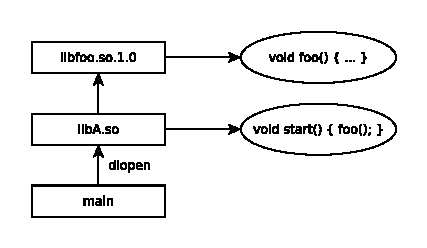
\includegraphics{figures/libdeps-ex1.pdf}
        \caption{Un exemple de dépendance de bibliothèques au sein d'un application simple fictive.
            La bibliothèque \textit{libA.so} est chargé dans l'application \texttt{main} via
            les appels au procédure \textit{dlopen} et \textit{dlsym}. Les fonctionnalités utilisés
            dans l'exemple sont marqué dans des ellipses.
        }
        \label{fig:deps-ex1}
    \end{figure}
\end{center}

Dans la situation situation présenté dans la figure-\ref{fig:deps-ex1}, quels sont les étapes inclus
dans l'exécution de ce programme qui invoque la fonctionnalité \texttt{start} de la
bibliothèque \textit{libA.so}. La fonctionnalité externe \texttt{start} est résolu de façon direct par
un appel à \verb|dlsym(libA, "start")|, qui commence la recherche de la procédure \texttt{start} dans
la bibliothèque spécifier dans \texttt{dlsym}. Le programme l'invoque une fois la procédure trouvée.
L'appel à une procédure non résolue (e.g.\ la procédure \texttt{foo} invoqué dans \texttt{start})
déclenche une procédure automatique de résolution des fonctionnalités. Cette procédure de résolution
commence sa recherche à partir de l'exécutable, puis itère la liste des dépendances directe. Si la
fonctionnalité n'est pas encore trouvé, la recherche continuera à partir de la bibliothèque passé à
\texttt{dlsym}.

% Stub

% TODO: exemple de résolution direct
Il est facile d'exploiter l'ordre de recherche du \textit{dynamic linker} pour
causer un masquage de fonctionnalité dans un application. Ce masquage est
utilisé dans certain contexte pour déboguer un programme, mais il peut aussi
nuire à l'exécution du programme. Il y au moins deux structures de programme
qui cause un masquage. L'application principale est construit comme une
bibliothèque dynamique exécutable et fournit une fonctionnalité qui porte le
même nom qu'une fonctionnalité exporté par une bibliothèque externe chargé
manuellement.  L'application principale est lié avec une bibliothèque qui
exporte une fonctionnalité qui porte le même nom que celle utilisée dans la
bibliothèque externe.

La figure-\ref{fig:deps-ex2} est un exemple de masquage qui utilise la seconde
méthode. La première méthode requière des bibliothèques exécutables qui n'est pas
disponible sur toutes les plateforme. Sous Linux, il est possible de créer une
bibliothèque exécutable en passant le paramètre \texttt{-rdynamic} à \textit{gcc}
lors de la construction.

\begin{center}
    \begin{figure}[ht]
        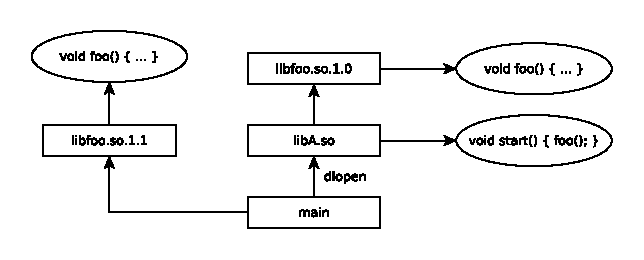
\includegraphics{figures/libdeps-ex2.pdf}
        \caption{Exemple de dépendance dans un application cause le masquage de la fonctionnalité \texttt{foo}
        de la bibliothèque \textit{libfoo.so.1.0} par la bibliothèque \textit{libfoo.so.1.1}}
        \label{fig:deps-ex2}
    \end{figure}
\end{center}
%% BEGIN
% D'autre langage compilé comme C/C++
% ne le permette pas directement, la liste des bibliothèques de code utilisé par un
% programme est déterminée lors de la création du fichier binaire, qui peut être
% soit un exécutable où une bibliothèque.
%% END


% TODO: pourquoi est-ce utile?
% XXX: structure pas final.
% - Les bibliothèques coexistent dans les application de tous les jours.
L'analyse des interactions entre des bibliothèques au sein d'un même programme permet de
mieux comprendre quels sont les circonstance qui peuvent conduire à des comportements
non désirés, comme le masquage de fonctionnalité présent l'exemple de la figure-\ref{fig:deps-ex2}.
Cela permet aussi d'établir les conditions qui permette d'éviter ces comportements non désirés.

\subsection{Coexistence entre les bibliothèques}

Les bibliothèques coexistent dans deux contexte principaux, de façon passive
dans un système fichier et de façon active durant l'exécution d'un programme.
Un système de fichier contient un arborescence hiérarchique de répertoires et
de fichiers avec une seule racine. Un fichier est l'entité dans un système de
fichier qui contient le code des bibliothèques.  Les répertoires sont les
entités qui permette de regrouper plusieurs fichiers de façon logique. La
racine correspond au sommet de la hiérarchie du système de fichier. La façon de
référer à un fichier dans un système de fichier est d'utiliser le
chemin absolu. Cela correspond à la liste des répertoires à parcourir de la
racine jusqu'au fichier. L'outil responsable d'organiser les bibliothèques sur
un système est le \textit{package manager}. Il a plusieurs objectif
incluant l'installation de bibliothèque, la mise à jour des
bibliothèques installées, la désinstallation de bibliothèque et la résolution
des dépendances.

Un cas intéressant de coexistence entre bibliothèques est celui qui inclue
plusieurs versions d'une bibliothèque. Les problèmes peuvent être liés à
d'organisation sur le système de fichier et au masquage de fonctionnalité
durant l'exécution d'un processus.  Il y a aussi plusieurs utilités de
conserver plusieurs version d'une bibliothèque, cela permet de supporter des
applications qui dépend de bibliothèques antérieurs.

Un autre application est de convertir un vieux format de fichier vers un format
plus récent. Dans le cas où il n'est pas possible de plusieurs version d'une bibliothèque
il faut alors écrire un \textit{reader} pour lire le vieux format manuellement ensuite le
utilise fonctions de la version cible de bibliothèque pour générer le nouveau format du fichier.
Cette solution à comme problème que le \textit{reader} est beaucoup moins testé que la
vielle version de la bibliothèque. Cela demande aussi de réécrire qu'est-ce qui à déjà été fait.

\begin{figure}[ht]
  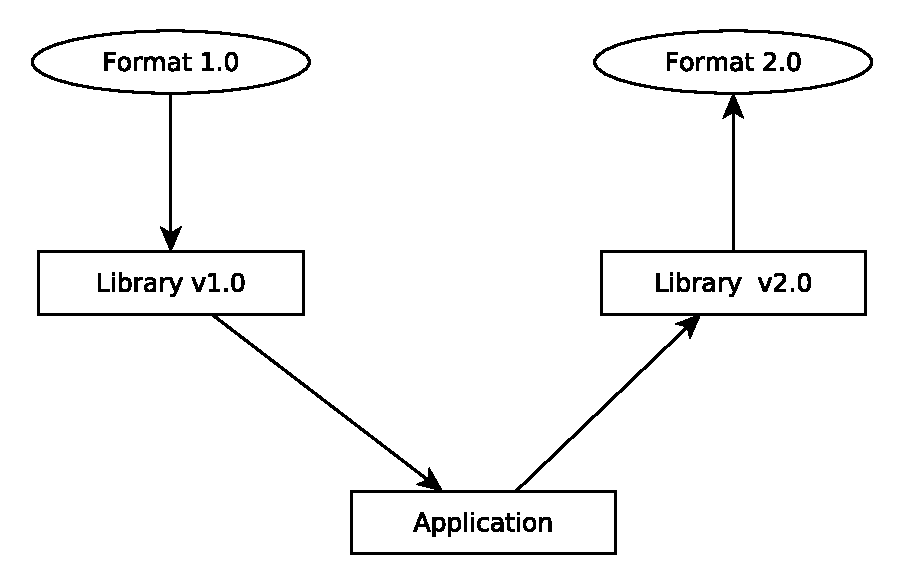
\includegraphics[width=30em]{figures/app_convert_v1_to_v2.pdf}
  \caption{Un exemple d'application de conversion entre deux version d'un format
  de fichier comme sqlite2 et sqlite3 exploitant la possibilité de charger plusieurs
  version d'une bibliothèque.}
\end{figure}

% L'architecture de processus sur un système permet plusieurs propriétés. La
% robustesse, un processus failli les autres processus ne sont pas affectés. La
% sécurité et l'isolation, chaque processus possède leur mémoire qui n'est pas
% accessible par les autre processus et peuvent utilisé une version spécifique
% des bibliothèques. Il est possible de concevoir l'architecture de processus en
% utilisant des threads.  Un \textit{thread} décrit un courant d'exécution d'un
% programme. Un processus à au minimum un \textit{thread} qui correspond au
% courant d'exécution principal du programme. Les \textit{threads} sont utiles
% pour paralléliser l'exécution d'un processus. La création de \textit{threads}
% est beaucoup plus rapide que la création d'un processus, car elle ne nécessite
% pas l'appel au système d'exploitation.

% Ce modèle exploite la légèreté des \textit{threads} par rapport au processus et
% la possibilité de charger plusieurs version des bibliothèques qu'il a besoin au sein
% du système. Cela est similaire au modèle de processus utilisé par les
% système d'exploitation, sauf que l'ensemble est juste au sein d'un seul processus.
% Étant donnée que les \textit{threads} vivent tous au sein d'un même processus,
% il est donc facile de partagé des informations d'un \textit{thread} à un autre.
% Ce qui est plus difficile avec le modèle de processus, cela nécessite l'utilisation
% mécanisme comme la mémoire partagé.

%\todo{picture: Thread as Light process}

% TODO: exemple de chemin.

%et s'il c'est un cas qui peut
%contenir un coexistence néfaste.  Cela n'est possible que s'il est possible de
%distinguer les deux version de la bibliothèque et aussi répartir les appels à
%des fonctions de même nom à la bonne version de la bibliothèque.

\section{Conditions entre des versions des bibliothèques}
%
Des conditions suffisantes pour que deux bibliothèques puissent coexister
ensemble au sein d'un processus incluant deux version de la même bibliothèque
est l'absence d'état global ou local, et l'unicité des nom des fonctionnalité.
L'absence d'état garantie que chaque fonction de la bibliothèque retourne
toujours un résultat prévisible dans un contexte identique. Un cas extrême est
la pureté fonctionnelle, qui est avantageux dans un contexte
\textit{multi-threadé}, car il n'est pas possible d'avoir une condition de
course sur une donnée partagé. La pureté fonctionnelle garantie qu'il n'y a pas
d'assignation.  Le fait que chaque fonctionnalité est associé à un nom unique
cela inhibe la capacité d'une bibliothèque de masquer une fonctionnalité d'une
autre bibliothèque.


% Une condition de courses survient lorsque l'ordre des opérations d'un programme
% s'exécute dans un ordre que le programmeur n'a pas conçu. Par exemple, un
% application avec deux fils d'exécutions, un qui lit la valeur d'une variable
% globales l'autre qui l'écrit.  Deux scénarios sont possible, la lecture peut
% s'effectuer avant ou après la la modification de la variable globale selon
% l'ordonnancement de ces deux fils d'exécution.  Le résultat de la lecture est
% dépendant de l'ordonnancement de ces deux opérations.

Ces conditions sont suffisante pour que deux bibliothèques coexiste sans
problème, mais elles ne sont pas nécessaires. Il existe des bibliothèques qui
ne respectent pas ces conditions, mais coexistent avec d'autres bibliothèques.
Pour tester la coexistence entre plusieurs bibliothèques, des expériences ont
été effectué dans plusieurs systèmes de modules existant. Le but de
l'expérience est d'observer le bon fonctionnement des la bibliothèques au sein
de même processus.

Les expériences qui suivent permette d'observer d'identifier les cas de cohabitation de bibliothèques
au sein d'un application qui cause des problème. Ils permettent aussi d'identifier les capacité d'un
langage à charger plusieurs versions d'une bibliothèques.

% XXX
%La capacité d'un langage d'interfacer avec d'autre langage via la FFI propage
%les limitations du langage cible.


\subsection{Bibliothèque C}
%
Les bibliothèques dans le langage C sont compilés dans un format natif pour la
plateforme courante (e.g. Window, MacOSX, Linux). Leur format diffère d'un
système d'exploitation à un autre, Window utilise le format \textit{dll}
(\textit{dynamic loading library}), MacOSX utilise le format \textit{dylib}
(\textit{Mach-O dynamic library}) et Linux utilise le format \textit{so}
(\textit{shared library}).

Les bibliothèques C consistent de symboles qui correspondent aux fonctions est
variables globales exportées. Une bibliothèque est généralement lié à un
programme C en lors de la création du programme. Les symboles non définis sont
résolus durant l'exécution du programme.

% TODO: complete
% - Bibliotheques avec collisions de nom de symboles
% - Masquage de fonctionnalité d'une des deux bibliothèque
Les collisions de symboles entre deux bibliothèques cause un masquage de
fonctionnalité d'une des deux bibliothèques. Un problème est de savoir si cela est
possible de chargé deux bibliothèque avec des collisions de symboles et accéder aux
fonctionnalités distincts de ces bibliothèques.

Pour chargé deux versions d'une même bibliothèque en C, il faut utilisé un
moyen qui prend en compte des symboles communs.  La résolution des symboles ce
fait par un parcourt en largeur dans la liste des symboles des bibliothèques.
Le résultat est le premier objet qui correspond au nom de symbole recherché.
L'ordre des bibliothèques utilisé dans la résolution des symboles correspond à
l'ordre spécifié lors de la construction de l'exécutable.

%    \vspace{-10pt}
\begin{center}
\begin{figure}[ht]
\begin{lstlisting}[frame=single]
> gcc -lSDL -lSDL2 exemple.c -o exemple
> ldd ./exemple
libSDL.so => /usr/lib/libSDL.so
libSDL2.so => /usr/lib/libSDL2.so
\end{lstlisting}
\caption{Création d'un exécutable lié aux deux bibliothèques
SDL et SDL2 dans cette ordre.}
\label{fig:sdl_mask_sdl2}
\end{figure}
\end{center}

La figure \ref{fig:sdl_mask_sdl2} donne la procédure de création d'un
exécutable lié avec deux versions de SDL.  Les tests ont été effectué sur deux
versions de SDL, 1.2 et 2, ils peuvent utiliser des ressources commune comme
les évènements du clavier, la mémoire et le GPU en utilisant OpenGL pour faire
de l'affichage 2D ou 3D.  Plusieurs situations sont testés, chacune sans thread
et avec des threads:
%
\begin{enumerate}
    \item Une utilisation de SDL minimaliste qui n'écoute pas les évènements utilisateurs.
    \item Une utilisation de SDL avec une boucle d'évènements de base.
    \item Une utilisation de SDL avec une utilisation d'un contexte OpenGL.
\end{enumerate}

%% SDL1.2 appel ces propres fonctions et SDL2 appel ces propres fonctions.
Puisque SDL1.2 et SDL2 on des collisions de symboles (i.e.\ \verb+SDL_Init+,
\verb+SDL_FillRect+, \verb+SDL_BlitSurface+, \dots), l'une des premiers
observations à effectuer est la bonne répartition des appels de fonctions des
deux bibliothèques dans le contexte d'une même application. Le problème à
identifier est un appels invalide à une procédure de SDL2 qui était destiné à
SDL1.2. Le facteur qui influence laquelle des deux bibliothèques va masquer
l'autre est l'ordre dans laquelle ils sont lié au programme à la création,
qui est montré à la figure-\ref{fig:sdl_mask_sdl2}.

Le masquage est une problématique qui peut mener à une défaillance du
programme, car cela peut provoquer la transmission d'une structure incompatible
de la première bibliothèque à la deuxième. Dans le cas de SDL, la structure
\verb+SDL_Surface+ à une disposition différente des champs, donc incompatible.
Le premier champ qui décale l'alignement de ces deux structures est le
\textit{pitch}, qui dans SDL1.2 est déclaré en Uint16 alors qu'en SDL2 il est
un int qui sont des types de taille différente. Donc, l'accès au prochain champ
\texttt{pixels} est différent entre SDL1.2 et SDL2, ce qui peut causer un accès
non désiré en mémoire si une structure de SDL1.2 est accédé comme une structure
de SDL2.

\begin{figure}[h]
  \centering
\begin{tabular}{p{18em}p{18em}}
\begin{lstlisting}[frame=single,numbers=left]
typedef struct SDL_Surface {
    Uint32 flags;
    SDL_PixelFormat *format;
    int w, h;
    Uint16 pitch;
    // Different offset here
    void *pixels;
    ...
} SDL_Surface;
\end{lstlisting}&
\begin{lstlisting}[frame=single,numbers=right]
typedef struct SDL_Surface {
    Uint32 flags;
    SDL_PixelFormat *format;
    int w, h;
    int pitch;
    // Different offset here
    void *pixels;
    ...
} SDL_Surface;
\end{lstlisting}\\
\end{tabular}
  \caption{C'est la comparaison entre la structure \textbf{SDL\_Surface} de SDL1.2 et SDL2 respectivement.}
  \label{fig:sdl_surface}
\end{figure}

%% Instable: gcc -lSDL -lSDL2 ...
Puisque les programmeurs cherchent une certaine stabilité dans leurs bibliothèques, ils ont
tendance à éviter les dépendances avec des bibliothèques qui ont des collisions de fonctionnalités.
Il est peu probable d'avoir une cohabitation entre deux bibliothèques avec des nom de fonctionnalités
similaires au sein.
% XXX: continue here

Le cas qui pourrait permettre plusieurs bibliothèques avec des collisions de symboles
au sein d'une même est avec l'API du \textit{dynamic linker}. Un teste simple permet
de démontrer la capacité de répartir les appels d'une fonction identifié par le même nom
dans différentes bibliothèques.

La structure générale des tests est organisé comme suit. Deux bibliothèques implémentant
une interaction valide avec l'une des versions de la bibliothèque (e.g. SDL1.2, SDL2).
Un application qui unie ces deux bibliothèques en utilisant l'API du
\textit{dynamic linker} pour exécuter ces deux bibliothèques séquentiellement ou
parallèlement.

%% TODO: expliquer la structure des programmes.

Dans le test minimaliste sans gestion d'évènements l'exécution des bibliothèque
fonctionne dans les deux cas, séquentiellement et en parallèle. La raison qui
explique ce bon fonctionnement est la répartition des appels au fonctions
des deux bibliothèques et le fait qu'il n'utilise pas de structure commune,
qui pourrait causer des conditions de course dans le test en parallèle.

\begin{center}
  \begin{figure}[ht]
\begin{lstlisting}[language=C,frame=single]
#include <SDL/SDL.h>

int main(int argc, char **argv) {
  SDL_Init(SDL_INIT_VIDEO);
  SDL_WM_SetCaption("sdl1_2", NULL);
  SDL_Surface *win =
    SDL_SetVideoMode(200, 200, 24, SDL_HWSURFACE);

  Uint32 color = SDL_MapRGB(win->format, 255, 0, 0);

  SDL_FillRect(win, NULL, color);
  SDL_Flip(win);
  SDL_Delay(1000);

  SDL_FreeSurface(win);
  SDL_Quit();
  return 0;
}
\end{lstlisting}
    \caption{Programme qui utilise la bibliothèque SDL1.2 sans la gestion des évènements
    Cette application génère une fenêtre rouge qui se ferme après 1 seconde de délais.}
  \end{figure}
\end{center}

%TODO: wrap these into frame
\begin{center}
  \begin{figure}[ht]
\begin{lstlisting}[language=C,frame=single]
#include <SDL2/SDL.h>

int main(int argc, char **argv) {
  SDL_Init(SDL_INIT_VIDEO);
  SDL_Window *win = SDL_CreateWindow("title",
      SDL_WINDOWPOS_CENTERED, SDL_WINDOWPOS_CENTERED,
      200, 200, SDL_WINDOW_SHOWN);
  SDL_Surface *screen = SDL_GetWindowSurface(win);

  Uint32 color = SDL_MapRGB(screen->format, 0, 255, 0);
  SDL_FillRect(screen, NULL, color);
  SDL_UpdateWindowSurface(win);
  SDL_Delay(1000);
  SDL_DestroyWindow(win);
  SDL_Quit();
  return 0;
}
\end{lstlisting}
    \caption{Programme qui utilise la bibliothèque SDL2 sans la gestion des évènements.
    Cette application génère fenêtre verte qui se ferme aussi après 1 seconde de délais.}
  \end{figure}
\end{center}

Dans le test incluant des évènements, l'hypothèse supposait que les évènements du clavier
aurait causé des problèmes de conditions de course en parallèle. Le test a aussi fonctionné
séquentiellement et en parallèle, malgré la dépendance commune du clavier.

Le test qui incluait OpenGL, n'aurait pas dû fonctionné par hypothèse. Les deux version
de SDL référait à une unique version de OpenGL. Le résultat a été surprenant, car le test
séquentielle et parallèle à fonctionné. Ce qui amène à conclure qu'il existe des cas
de coexistence entre des bibliothèques avec des collisions de symbole qui fonctionne
sans causer des problèmes d'exécution.



%%% Possible de compile le programme principale en un exécutable et en bibliothèque.
%Les deux programmes sont compilés en bibliothèques et en exécutables.
%Le fonctionnement de chaque programme est testé de façon séparé.
%Le programme principale, qui charge le main des deux autres programmes en utilisant
%l'API du \textit{dynamic loader}, est compilé en mode séquentiel et en mode parallèle.
%La version séquentielle permet d'observer la coexistance entre les deux bibliothèques,
%celle parallèle est utilisé pour évaluer les conditions de course sur des ressources
%communes.
%
%%% TODO: schema.
%\begin{center}
%  \begin{figure}[ht]
%\begin{lstlisting}[language=C,frame=single]
%  ...
%  void *hndl1 = dlopen(prog1, RTLD_NOW);
%  void *hndl2 = dlopen(prog2, RTLD_NOW);
%
%  int(*main1)(int,char**) = dlsym(hndl1, "main");
%  int(*main2)(int,char**) = dlsym(hndl2, "main");
%
%  main1(argc, argv);
%  main2(argc, argv);
%  ...
%\end{lstlisting}
%  \caption{Le chargement et exécution séquentiel de la fonction main des programmes
%  \textbf{prog1} et \textbf{prog2} via l'API du \textit{dynamic loader}.}
%  \end{figure}
%\end{center}
%% \begin{center}
%%   \begin{figure}[ht]
%% \begin{lstlisting}[language=C,frame=single]
%% struct MainCallback {
%%   int argc;
%%   char **argv;
%%   int (*main)(int,char**);
%% };
%%
%% void *run(void* args) {
%%   struct MainCallback* callback = (MainCallback*)args;
%%   callback->main(callback->argc, callback->argv);
%%   return NULL;
%% }
%% \end{lstlisting}
%%   \caption{Callback utilisé pour exécuté le main de la bibliothèque chargé par
%%   \textbf{dlsym} en parallèle avec pthread.}
%%   \end{figure}
%% \end{center}
%
%\begin{center}
%  \begin{figure}[ht]
%\begin{lstlisting}[language=C,frame=single]
%  ...
%  struct MainCallback callback = {
%    .argc = argc,
%    .argv = argv,
%    .main = main1
%  };
%
%  pthread_t th1;
%  pthread_create(&th1, NULL, run, &callback);
%  main2(argc, argv);
%  pthread_join(th1, NULL);
%  ...
%\end{lstlisting}
%    \caption{Exécution du code des deux programme en parallèle avec l'utilisation de pthread.
%    Contrairement à la figure précédente, la fonction main de \textbf{prog1} exécuté dans un
%    threads.}
%  \end{figure}
%\end{center}
%
%
%Tout d'abord, la compatibilité entre SDL1.2 et SDL2 à été testé par un code sans
%la gestion des évènements, pour vérifier si les fonctions respective de chaque
%bibliothèque étaient à appellé correctement.
%% coexistance sans interraction directe.
%#ifdef THREADED

% SDL1.2/SDL2/OpenGL
% - Hypothèse
%   - Non-threaded without OpenGL
%   - Non-threaded with OpenGL
%   - Threaded without OpenGL
%   - Threaded with OpenGL
% - Démarche
% - Résultat
% - Petite Conclusion

% OpenSSL+RSA/OpenSSL+Socket
% - Hypothèse
% - Démarche
% - Résultat
% - Petite Conclusion

\clearpage
\subsection{Bibliothèque Scheme avec FFI}
La compatibilité entre version a été testé sur la partie cryptographique
RSA de OpenSSL, SDL et un générateur aléatoire qui possède un état global.
Pour observer le comportement de bibliothèque Scheme liant des fonctionnalités
implémenté dans un autre langage, dans ces exemple C. Ces tests montrent le problème
de masquage décrit précédemment dans des bibliothèques réelle.
Pour tester les bibliothèques natives en Scheme, il a fallut écrire des
un code spécial pour lier les types et les fonction au monde Scheme. Ces

Par hypothèse la partie cryptographique des deux versions de OpenSSL peuvent
coexister. Chacune des fonctions cryptographique de OpenSSL1.0 et OpenSSL1.1
exécute du code disjoint qui n'interfère pas avec une zone mémoire commune.
Cela implique qu'un appelle à une fonction de OpenSSL1.0 n'affectera pas les
résultats des appelles futures de OpenSSL1.1. Les fonctions nécessaires
pour tester la partie cryptographique RSA sont:
\begin{itemize}
    \item \lstinline{PEM_read_bio_RSA_PUBKEY} et \lstinline{PEM_read_bio_RSAPrivateKey}:
        Ce sont les fonctions OpenSSL qui permettent de lire la clef publique et la clef privée.
    \item \lstinline{RSA_public_encrypt}:
        La fonction d'encryption qui crypte un  message en utilisant une clef publique.
    \item \lstinline{RSA_private_decrypt}:
        La fonction qui permet de décrypter un message en utilisant la clef privée.
    \item \lstinline{RSA_free}:
        La fonction qui libère la mémoire alloué pour les clefs publiques et privées.
        Cette fonction n'est pas nécessaire pour les testes, mais utile pour une bonne
        gestion mémoire.
\end{itemize}
La structure de donnée utilisé par les fonctions d'OpenSSL pour la cryptographie RSA
est un pointeur vers un enregistrement RSA. La liaison avec le type C est effectué avec
la forme spécial \lstinline{c-define-type}.

Le teste consiste à crypter un message en utilisant une clé publique, décrypter le
cryptogramme avec la clé privée et comparer le message original avec le message décrypter
pour les deux versions de OpenSSL chargé dans le même processus. Pour vérifier la bonne
invocation des fonctions de OpenSSL1.0 et OpenSSL1.1 respectif le débogueur \textbf{gdb}
a été utilisé. Les bibliothèques d'OpenSSL consiste en deux fichier \url{libssl.so} et \url{libcrypto.so}.
En déboguant la répartition des appels avec \textit{gdb}, il y a eu l'observation que
la bibliothèque \url{libcrypto.so} de OpenSSL1.1 masquait la version de OpenSSL1.0 s'il
n'est pas spécifié explicitement lors de la création de la bibliothèque Scheme \textit{rsa.scm}
comme à la figure-\ref{fig:scm_masq1}. Les raisons sont liées à plusieurs facteurs qui étaient présents
durant l'expérience. L'ordre de recherche des symboles qui inclue les symboles des bibliothèques lié à
l'exécutable qui sont prioritaire qui contenait \url{libssl.so} et \url{libcrypto.so} de OpenSSL1.1.
Dans ce cas, il était possible de résoudre ce problème en ajoutant une
dépendance directe à \textit{libcrypto} lors de la construction des bibliothèques Scheme \verb+RSA+
comme montré dans la figure-\ref{fig:scm_masq_fix1}.

\begin{center}
\begin{figure}[ht]
\begin{lstlisting}[frame=single]
gsc-script -o rsa-1-0-0.o1 \
  -cc-options '-I /usr/include/openssl-1.0' \
  -ld-options '-L /usr/lib/openssl-1.0 -lssl' \
  -prelude '(define-cond-expand-feature|openssl-v10|)' rsa.scm

gsc-script -o rsa-1-1-0.o1 \
  -ld-options "-lssl" rsa.scm
\end{lstlisting}
\caption{Création des bibliothèques \textit{rsa.scm} pour OpenSSL1.0 et OpenSSL1.1
sans la spécification de \textit{libcrypto.so}}
\label{fig:scm_masq1}
\end{figure}
\end{center}

\begin{center}
\begin{figure}[ht]
\begin{lstlisting}[frame=single]
gsc-script -o rsa-1-0-0.o1 \
  -cc-options '-I /usr/include/openssl-1.0' \
  -ld-options '-L /usr/lib/openssl-1.0 -lssl -lcrypto' \
  -prelude '(define-cond-expand-feature|openssl-v10|)' rsa.scm

gsc-script -o rsa-1-1-0.o1 \
  -ld-options "-lssl -lcrypto" rsa.scm
\end{lstlisting}
\caption{Création des bibliothèques \textit{rsa.scm} pour OpenSSL1.0 et OpenSSL1.1
avec la spécification de \textit{libcrypto.so}}
\label{fig:scm_masq_fix1}
\end{figure}
\end{center}

\begin{center}
\begin{figure}[ht]
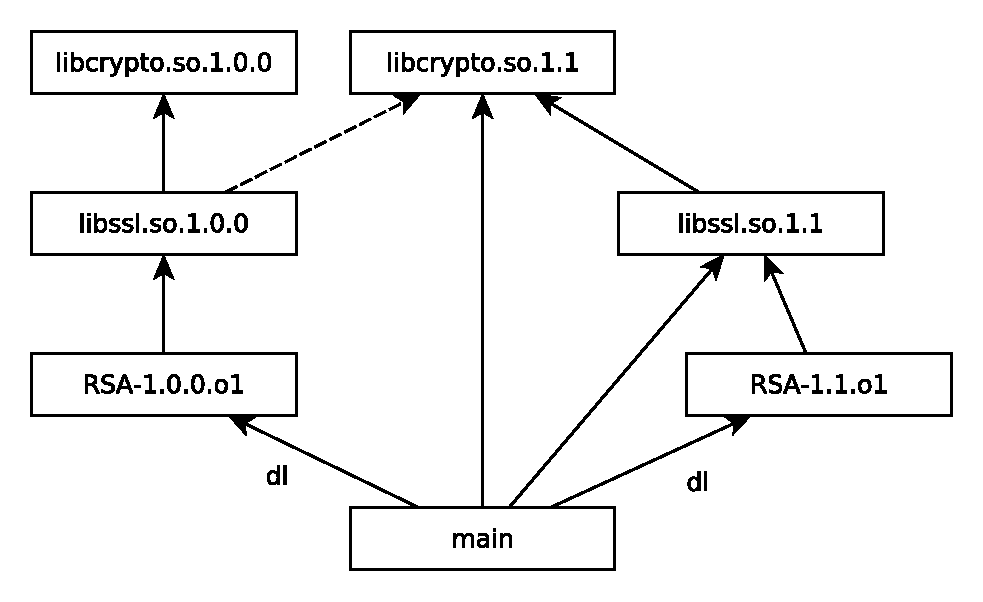
\includegraphics{figures/libssl_masking.pdf}
\caption{Schéma des dépendances entre les bibliothèques au sein d'un processus.
Les dépendances qui ont été lié dynamiquement lors la création de l'application sont représenté par une flèche avec
trait plein sans annotation. Ceux qui représente les chargement de bibliothèque dynamique via \texttt{dlopen} ont
l'annotation \textit{dl}. La flèche en pointillé indique un masquage des symboles de la bibliothèque
source par celle pointée.}
\label{fig:scm_masq_schema}
\end{figure}
\end{center}

TODO: rng générator

%\begin{lstlisting}[frame=single]
%(c-define-type RSA* (pointer "RSA"))
%\end{lstlisting}


%Heureuse Gambit Scheme possède un interface pour lié
%une fonction C au monde Scheme.

%Une bibliothèque liant les fonctions principales de SDL au monde Scheme.


%\TODO{Fill}
% SDL / SDL2
% - Hypothèse
% - Démarche
% - Résultat
% - Petite Conclusion

% OpenSSL+RSA
% - Hypothèse
% - Démarche
% - Résultat
% - Petite Conclusion

% RNG-splitmx64/RNG-xoroshiro128+
% - Hypothèse
% - Démarche
% - Résultat
% - Petite Conclusion


\subsection{Bibliothèque Javascript (NodeJS)}
%\TODO{Fill}
% Démarche général
% express / sqlite3
% - Hypothèse * 2
% - Démarche/Expérimentation
% - Résultat
% - Petite Conclusion

Pour effectué des tests sur la coexistences de différente version d'une bibliothèque
Javascript dans NodeJS, il faut tout d'abord permettre l'importation de plusieurs
versions d'une même bibliothèque. Dans NodeJS, l'importation de module s'effectue
avec la fonction \verb|require(module-name)|. Puisque l'information de version
de la bibliothèque n'est pas fournit en paramètre à la fonction, il faut donc
utilisé une autre méthode de forcer plusieurs versions des bibliothèque.
La configuration d'un module dans NodeJS utilise le format JSON pour spécifier
le nom, la version, les dépendances, \dots.

Les dépendances sont conservées sous la forme d'un arbre, chaque module à ses dépendances directes
qui ont aussi des dépendances indirectes.  Lors de l'écriture d'un module Javascript, il est possible
de spécifier la version de chaque dépendence dans le fichier \textit{package.json}.
\begin{verbatim}
{
  ...
  "dependencies": {
    "express": "4.16.3"
  },
  ...
}
\end{verbatim}
En utilisant cette fonctionnalité du système de module de NodeJS, deux bibliothèques \textit{wrapper}
sont écrit pour interfacer les deux versions de express. Puisque l'API public d'express n'a pas changé entre
les versions 3.21.1 et 4.16.3, il est possible de recycler le code de la bibliothèque qui encapsule une
version d'express (figure-\ref{fig:express}).
\begin{center}
\begin{figure}[ht]
    % FIXME: language=Javascript
    \begin{lstlisting}[language=C,frame=single]
const express = require('express');

function start() {
  const app = express();
  const port = Math.floor(Math.random() * 64535 + 1000);

  app.get('/', (req, res) => {
    res.send('Hello world!\n');
  });

  app.listen(port, 'localhost', () => {
    console.log('Listen on port ' + port);
  });
}
exports.start = start;
\end{lstlisting}
\end{figure}
\label{fig:express}
\end{center}
Le programme principale ne fait qu'importer les deux encapsulation de bibliothèque
et invoque la fonction \textit{start}.

Le résultat attendu dans cette expérience est que ces deux version de la bibliothèque
express coexiste sans problème, sauf dans le cas où le port tcp utilisé par les deux
version est le même. Dans ce cas, c'est la bibliothèque dont la fonction
\textit{start} a été invoqué en premier qui va monopoliser le tcp port. Dans ce cas
la ressource qui inhibe la coexistence de ces modules au sein d'un même processus
est lié au \textit{socket}.

\subsection{Variables globales communs}

Puisque qu'il n'existe qu'une seul instance de chaque bibliothèque en mémoire, cela implique
que les variables globale d'une bibliothèque.

Définissons 3 bibliothèques B, C et D telle que D a une variable globale nommée \textit{value}.
B et C ont chacun une dépendance directe vers D, et exportent une référence de la variable
globale \textit{value} de D.

Le programme principale A commence par charger B et C. Ensuite lit la valeur de \textit{B.D.value}
puis modifie \textit{C.D.value} et relit \textit{B.D.value}. Le teste réussi si la valeur de
\textit{B.D.value} reste inchangé par la modification de \textit{C.D.value}. Cela implique que
les références vers la bibliothèque D est différente de via B et via C.

Dans NodeJS, un module peut être installé via un dossier, un archive tarball, un dépôt de code source git ou
directement via Npmjs. Puisque un module publié dans Npmjs ne peut pas être retiré facilement étant donné
la politique lié au module (\url{https://docs.npmjs.com/cli/unpublish}).
%L'expérience va utilisé un serveur git qui est auto-hébergé.
